\documentclass[10pt,a4paper]{article}
\usepackage[margin=2cm]{geometry}
\usepackage{amsmath,amssymb,booktabs,graphicx,caption,xcolor,float,hyperref,tikz}
\usetikzlibrary{arrows.meta,positioning,calc}
\hypersetup{colorlinks=true,linkcolor=blue!50!black,urlcolor=blue!50!black}
\captionsetup{font=small,labelfont=bf}
\title{\vspace{-1.2cm}\textbf{A larger budget, a board that forgets faster or slower}\\[2pt]
\large Simulation 2 (asynchronous activation), setup \texttt{task003-symmetric}: three variants against the gold standard}
\author{LLM-free simulator; report of 19 October 2026; runs of 15, 16 and 18 October 2026\\
\small Same sections, figures and equations as the gold-standard report of 16 October, with the four cases side by side.}
\date{}
\begin{document}
\maketitle
\vspace{-1cm}

\paragraph{How the simulator works.} The world, \texttt{task\_003}, has three candidate allocations; A0 is the
correct one. Each of 24 agents is given one true fact and reasons as an exact Bayesian: its \emph{belief} is the
exact probability of A0, A1 and A2 given the facts it currently remembers. There are no rounds. Each agent acts
at random times, on average once per time unit: it reads $q$ posts drawn at random from the $W$ most recent posts ($W = 48$ in the gold standard)
on a shared \emph{board} (never its own), adds their facts to its memory, recomputes its belief, \emph{votes} by
probability matching (a vote drawn from its belief) and posts one remembered fact that supports its vote. Every
remembered fact is forgotten after a random lifetime (on average a fraction $\rho$ survives one time unit; reading
it again renews it). A \emph{controller} with a target, A0 (truth) or A2 (false), acts at random times at rate
$\lambda_c$ until $t = 30$: it reads $q_c$ recent agent posts and, unless the \emph{vote gate} (at least 75\% of
them from agents voting for its target) or the \emph{proof stop} (its target already proved) silences it, posts
the one fact from its pool that best supports its target, at most $B$ messages per episode ($B = 30$ in the gold standard). Agents continue
alone until $t = 40$. Every episode is run three times with the same random draws: without a controller
(\emph{silent}), with the controller targeting A0 and with the one targeting A2.

\paragraph{The facts at the start.} All facts are true. The agents hold, together, a proof of A0; no single
agent does, and neither pool can prove its target (Table~\ref{tab:facts}).

\begin{table}[H]
\centering\small
\caption{Facts available at $t = 0$ and what each set implies, $P(\text{A0}, \text{A1}, \text{A2} \mid \text{facts})$.}
\label{tab:facts}
\begin{tabular}{lcc}
\toprule
set of facts & facts & $P(\text{A0}, \text{A1}, \text{A2})$ \\
\midrule
agents' facts, all together (24 agents, one fact each) & 18 distinct & (1, 0, 0): proves A0 \\
A0 pool (controller with target A0) & 12, of which 10 new to the agents & (0.963, 0.037, 0) \\
A2 pool (controller with target A2) & 12, of which 10 new to the agents & (0.114, 0, 0.886) \\
agents' facts + either pool & 28 distinct & (1, 0, 0) \\
\bottomrule
\end{tabular}
\end{table}

\paragraph{The three variants.} Each changes one rule of the gold standard and keeps everything else
(Table~\ref{tab:cases}).

\begin{itemize}\itemsep1pt
\item \textbf{Budget.} In the gold standard the controller may post at most $B = 30$ messages before $t = 30$; from
  $\lambda_c = 2$ upward it uses almost all of them, and at $\lambda_c = 8$ it runs out near $t = 4$. With $B = 100$
  it can keep posting until $t = 30$ for $\lambda_c \lesssim 3$ and runs out near $t = 12.5$ at $\lambda_c = 8$; the
  vote gate can still silence it. This separates the rate from the total effort.
\item \textbf{Board window.} Nothing is ever deleted from the board, but every reader (agent or controller) draws
  only from the $W$ newest posts it may read. The 24 agents post about 24 times per time unit, so in the gold
  standard ($W = 48$) a post stays readable for about 2 time units unless someone posts its fact again. With
  $W = 24$ it stays about 1 time unit (a board that forgets fast); with $W = 240$ about 10 (a board that forgets
  slowly). The window also changes what the controller reads, so with $W = 240$ its vote gate sees older votes.
\end{itemize}

\begin{table}[H]
\centering\small
\caption{The four cases compared in this report. All: $q_c = 12$, $\rho \in \{1, 0.75, 0.5, 0.25\}$, $q \in \{3, 6, 12\}$,
all nine rates, gate on and off, 1{,}000 episodes per setting.}
\label{tab:cases}
\begin{tabular}{lccll}
\toprule
case & budget $B$ & window $W$ & a post stays readable & run \\
\midrule
gold standard & 30 & 48 & $\approx 2$ time units & 15--16 October (\texttt{*\_fine}) \\
$B = 100$ & 100 & 48 & $\approx 2$ & 18 October (\texttt{*\_budget100}) \\
$W = 24$ & 30 & 24 & $\approx 1$ & 18 October (\texttt{*\_window24}) \\
$W = 240$ & 30 & 240 & $\approx 10$ & 18 October (\texttt{*\_window240}) \\
\bottomrule
\end{tabular}
\end{table}

\paragraph{The runs.} The gold standard's settings at $q_c = 12$ and $\rho \in \{1, 0.75, 0.5, 0.25\}$ (from the
15--16 October runs) and the three variants on the same grid: posts read by an agent $q \in \{3, 6, 12\}$; rate
$\lambda_c \in \{0.5, 1, 2, 3, 4, 5, 6, 7, 8\}$; vote gate on and off; proof stop on; 1{,}000 episodes per setting
(444 settings per case). Unless stated otherwise: $q = 6$, $q_c = 12$, $\lambda_c = 1$, gate on. Where the budget
cannot matter, the $B = 100$ run reproduces the gold standard exactly: all silent settings, and every setting in
which the gold-standard controller never reached 30 messages (113 settings).

\paragraph{How this report is organised.} Part~A (Section~\ref{sec:budget}) compares the gold standard with
$B = 100$; Part~B (Section~\ref{sec:window}) compares it with $W = 24$ and $W = 240$. Each part has the gold standard's
sections. Only the false controller (target A2) is shown: the controller targeting A0 changes by at most 0.03 in
every variant. Readability $I$ and efficiency $\eta$ still use both targets, as defined in Section~\ref{sec:quantities}.

\paragraph{Summary.} \textbf{The gold standard's main results hold in all three variants}: full memory makes the
swarm immune, forgetting makes it steerable, and reading more protects when agents remember and helps the controller
when they forget. \textbf{A budget of 100 messages lets fast controllers keep gaining} (Part~A): up to $+0.13$ at
$\rho \le 0.5$, with each extra message worth about half as much; the 30-message cap is what made the rate look
irrelevant to the end point. \textbf{The board's memory protects like the agents' memory, but less} (Part~B): posts
that stay readable for 10 time units instead of 2 lower the false controller's gain by 0.06--0.14 at $\rho \le 0.5$;
posts readable for 1 time unit raise it by up to 0.09.

\section{Quantities}\label{sec:quantities}

\paragraph{Votes.} With $n_{a,t}$ the number of agents whose last vote is answer $a$ at time $t$ and $N_t$ the
number of agents who have voted,
\begin{equation}\label{eq:share}
x_{a,t} = n_{a,t}/N_t .
\end{equation}
At $t = 0$ nobody has voted and we set $x_{a,0} = 0$; all agents have voted by $t \approx 5$. (The 9--14 October reports divided by 24, which counted agents who had
not yet acted as voting against the target; this inflated the apparent rise of the shares and the apparent bias of
the controller's sensing at early times.)

\paragraph{Paired susceptibility.} Following \texttt{BLACKBOARD\_OBSERVABLES\_AND\_EFFICIENCIES} (\S3), for a
controller policy $\pi$ and an answer $a$,
\begin{equation}\label{eq:chi}
\chi^{(a)}_{\pi,t} \equiv G^{(a)}_t(\pi) = \mathbb E\bigl[x^{\pi}_{a,t} - x^{\rm base}_{a,t}\bigr],
\end{equation}
the mean over episodes of the difference between the controlled run and the silent run of the same episode. We
report it on the controller's own target: $G_t \equiv G^{(0)}_t(\pi^{+})$ for the controller targeting A0 and
$G_t \equiv G^{(2)}_t(\pi^{-})$ for the one targeting A2.

\paragraph{Target and state.} The target $Z \in \{\text{A0}, \text{A2}\}$ is drawn by a fair coin. The state $X$
at time $t$ is the vote of a randomly chosen agent, $X \in \{\text{A0},\text{A1},\text{A2}\}$. Each episode $e$ of arm $s$
(silent 0, target A0 $+$, target A2 $-$) contributes its vote shares $y^{(e)}_s(x) = x_{x,t}$, and
\begin{equation}\label{eq:P}
P_s(x) = \frac1E\sum_{e=1}^{E} y^{(e)}_s(x), \qquad E = 1000 .
\end{equation}

\paragraph{Readability and efficiency.} With $Q = \frac12(P_+ + P_-)$ and $\mathrm{KL}(p\Vert q) = \sum_x p(x)\log_2[p(x)/q(x)]$,
\begin{equation}\label{eq:I}
I(Z;X) = \tfrac12\,\mathrm{KL}(P_+\Vert Q) + \tfrac12\,\mathrm{KL}(P_-\Vert Q),
\end{equation}
the information the state carries about the target (at most 1 bit). The controllers' total change from silence
splits exactly into a directed and an undirected part,
\begin{equation}\label{eq:C}
C = \tfrac12\,\mathrm{KL}(P_+\Vert P_0) + \tfrac12\,\mathrm{KL}(P_-\Vert P_0) = I(Z;X) + \mathrm{KL}(Q\Vert P_0),
\end{equation}
and the efficiency is the directed share,
\begin{equation}\label{eq:eta}
\eta = I(Z;X)/C .
\end{equation}
Silence sometimes never shows a value of $X$ that a controller reaches, which would make $C$ infinite. Before
computing any KL, every arm's distribution therefore receives the same pseudo-count of $\alpha = 0.5$ episodes per
value of $X$ ($K$ values),
\begin{equation}\label{eq:smooth}
\tilde P_s(x) = \frac{E\,P_s(x) + \alpha}{E + \alpha K}.
\end{equation}
With $\alpha = 1$ instead, $\eta$ changes by at most 0.004; without it, by at most 0.005 where $C$ is finite. $\eta$ is not defined when $C < 0.01$ bits (no measurable change);
such values are left blank. Equation~(\ref{eq:C}) holds in the data to $4\times10^{-15}$ bits.

\paragraph{Cost.} $F_t$ is the number of facts the controller has posted up to $t$ (mean per episode); the gain
per fact is $G_t/F_t$, and the marginal susceptibility is the slope between neighbouring rates,
\begin{equation}\label{eq:slope}
\frac{\Delta G}{\Delta\lambda_c} = \frac{G(\lambda_c^{(k+1)}) - G(\lambda_c^{(k)})}{\lambda_c^{(k+1)} - \lambda_c^{(k)}} .
\end{equation}
Episode $e$ uses the same random draws at every rate, so the slope is estimated from per-episode differences,
$[x^{(e)}_{\text{target},t}(\lambda_c^{(k+1)}) - x^{(e)}_{\text{target},t}(\lambda_c^{(k)})]/(\lambda_c^{(k+1)} -
\lambda_c^{(k)})$, whose mean is Eq.~(\ref{eq:slope}) and whose standard error gives the 95\% intervals (typically
$\pm0.01$--$0.03$, about 30\% narrower than for two independent means).

%=====================================================================================================================
\section{Part A: a larger budget ($B = 100$)}\label{sec:budget}

The gold standard ($B = 30$) against $B = 100$; the window is $W = 48$ in both.

\subsection{Votes over time}

\begin{figure}[H]
\centering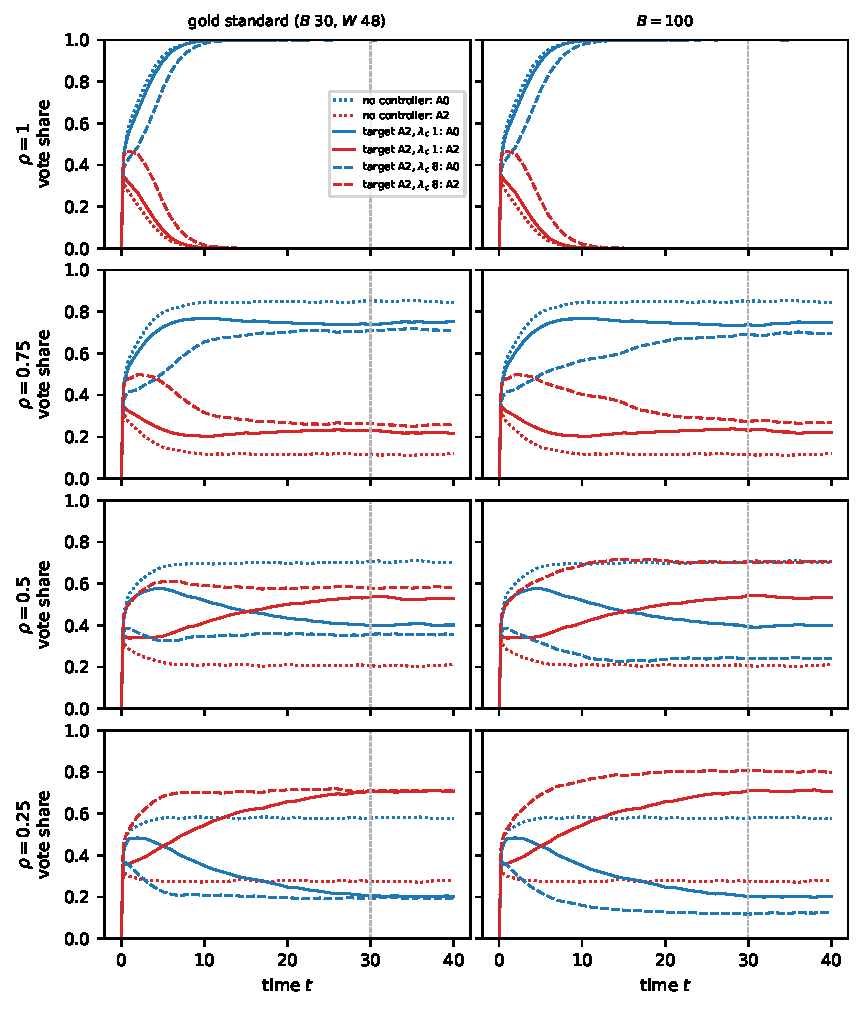
\includegraphics[width=0.55\linewidth]{figures/fig_votes_budget.pdf}
\caption{Share of agents voting A0 (blue) and A2 (red), Eq.~(\ref{eq:share}): without a controller (dotted) and with
the false controller (target A2) at $\lambda_c = 1$ (solid) and $\lambda_c = 8$ (dashed). Rows: memory $\rho$. $q = 6$,
$q_c = 12$, gate on. At $t = 0$ nobody has voted and every share is 0.}
\label{fig:votesB}
\end{figure}

\begin{itemize}\itemsep1pt
\item \textbf{At $\lambda_c = 1$ nothing changes}: the controller rarely reaches 30 messages, so the curves equal the gold
  standard's.
\item \textbf{At $\lambda_c = 8$ the false controller wins more votes where the swarm forgets}: A2 on $t = 30$ goes from
  0.58 to 0.70 ($\rho = 0.5$) and from 0.71 to 0.81 ($\rho = 0.25$); at $\rho = 0.75$ from 0.26 to 0.28; at $\rho = 1$ it is
  0 in both. The results persist to $t = 40$.
\end{itemize}

\subsection{Susceptibility over time, and per message}

\begin{figure}[H]
\centering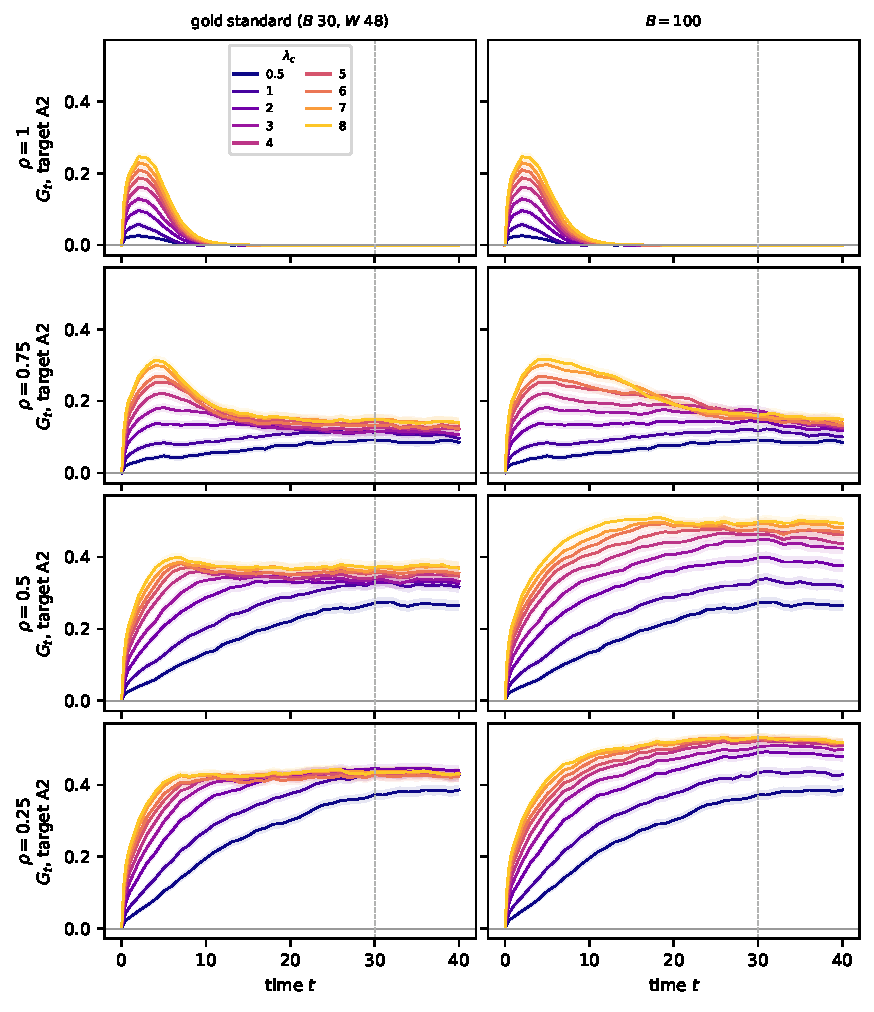
\includegraphics[width=0.55\linewidth]{figures/fig_gain_time_budget.pdf}
\caption{Paired susceptibility $G_t$, target A2, Eq.~(\ref{eq:chi}), one curve per rate $\lambda_c$ (bands: 95\%
intervals). Rows: $\rho$.}
\label{fig:gainB}
\end{figure}

\begin{figure}[H]
\centering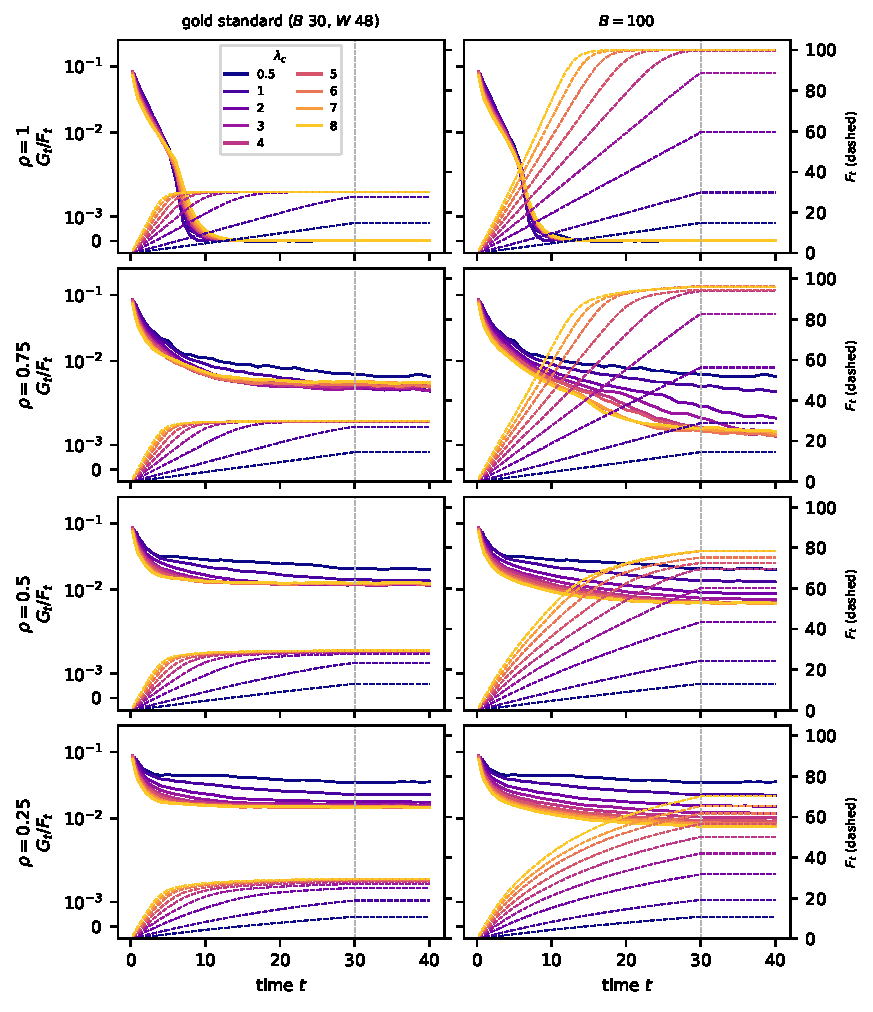
\includegraphics[width=0.55\linewidth]{figures/fig_per_fact_budget.pdf}
\caption{Gain per message $G_t/F_t$ (solid, left axis, log scale) and messages posted $F_t$ (dashed, right axis),
target A2, one colour per rate.}
\label{fig:perfactB}
\end{figure}

\begin{itemize}\itemsep1pt
\item \textbf{Fast controllers keep gaining after the gold standard's budget would have run out}
  (Figure~\ref{fig:gainB}): on $t = 30$, $G$ ranges over the rates from 0.27 to 0.50 at $\rho = 0.5$ (gold standard
  0.27--0.37) and from 0.37 to 0.53 at $\rho = 0.25$ (0.37--0.45); at $\rho = 0.75$ it rises by at most 0.06, at
  $\rho = 1$ not at all.
\item \textbf{Readability follows} (Figure~\ref{fig:phaserxB}, middle): on $t = 30$, $\rho = 0.5$, $I = 0.15$--$0.38$ bits
  against 0.15--0.27. \textbf{The efficiency drops a little} (right): $\eta = 0.76$--$0.91$ against 0.82--0.93 at
  $\rho < 1$.
\item \textbf{Each extra message is worth about half as much} (Figure~\ref{fig:perfactB}): on $t = 30$, $\lambda_c = 8$,
  $0.0063$ per message against $0.0126$ at $\rho = 0.5$ (78 messages against 29), $0.0076$ against $0.0148$ at
  $\rho = 0.25$.
\end{itemize}

\subsection{Phase diagrams}

\begin{figure}[H]
\centering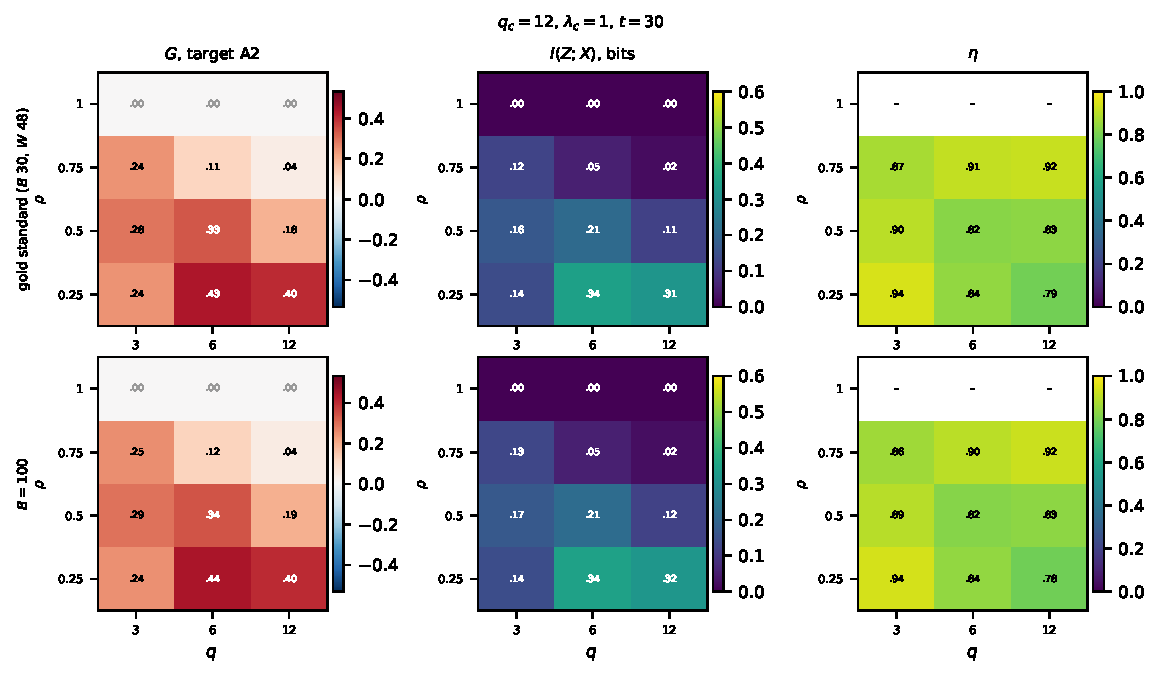
\includegraphics[width=0.9\linewidth]{figures/fig_phase_rho_q_budget.pdf}
\caption{Susceptibility (target A2; grey number: 95\% interval includes 0), readability and efficiency on $t = 30$
over memory $\rho$ and the posts each agent reads $q$. $q_c = 12$, $\lambda_c = 1$, gate on.}
\label{fig:phaserqB}
\end{figure}

\begin{figure}[H]
\centering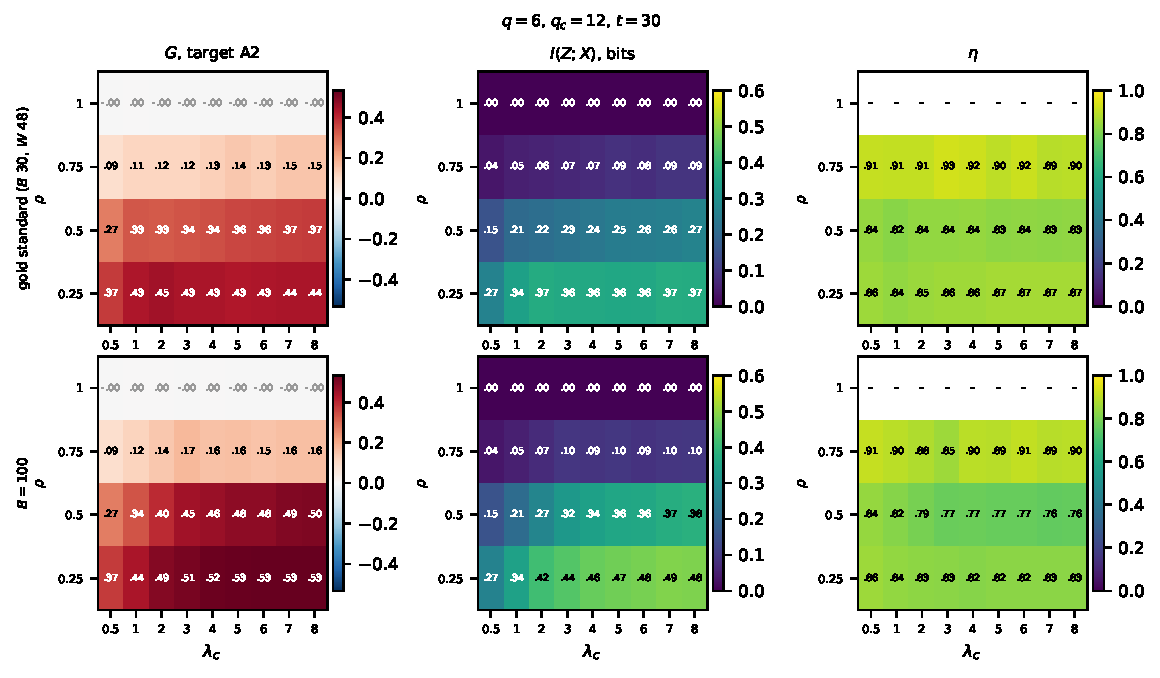
\includegraphics[width=0.9\linewidth]{figures/fig_phase_rho_x_budget.pdf}
\caption{The same over memory $\rho$ and the rate $\lambda_c$. $q = 6$, $q_c = 12$.}
\label{fig:phaserxB}
\end{figure}

\begin{itemize}\itemsep1pt
\item \textbf{At $\lambda_c = 1$ the reading reversal is unchanged} (Figure~\ref{fig:phaserqB}): reading more protects
  at $\rho = 0.75$ ($G$ 0.25 $\to$ 0.04 from $q = 3$ to 12) and helps the controller at $\rho = 0.25$ (0.24 $\to$ 0.40).
\item \textbf{The budget adds a rate gradient} (Figure~\ref{fig:phaserxB}): from $\lambda_c = 1$ to 8, $G$ grows by
  0.16 ($\rho = 0.5$) and 0.10 ($\rho = 0.25$), against 0.04 and 0 in the gold standard.
\end{itemize}

\subsection{Susceptibility against the rate, against messages, and its slope}

\begin{figure}[H]
\centering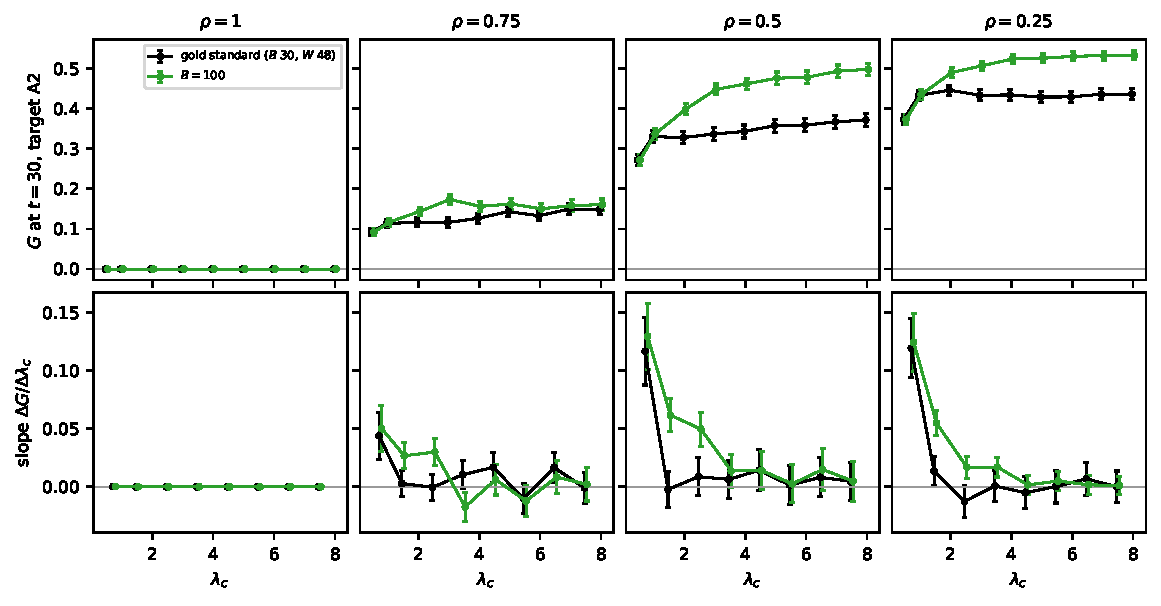
\includegraphics[width=0.98\linewidth]{figures/fig_gain_rate_budget.pdf}
\caption{Top: $G$ on $t = 30$, target A2, against the rate (bars: 95\% intervals). Bottom: the slope between
neighbouring rates, Eq.~(\ref{eq:slope}), with paired 95\% intervals. $q = 6$, $q_c = 12$, gate on.}
\label{fig:strengthB}
\end{figure}

\begin{figure}[H]
\centering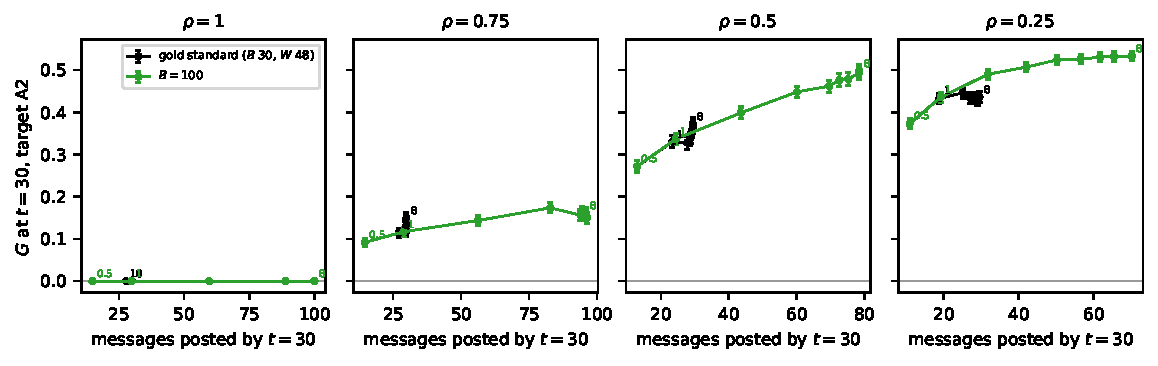
\includegraphics[width=0.98\linewidth]{figures/fig_gain_messages_budget.pdf}
\caption{$G$ on $t = 30$, target A2, against the messages posted by then; one point per rate, joined in rate order
(labels: $\lambda_c$ = 0.5, 1, 8); bars: 95\% intervals. Read it like Figure~9 of the 19 October gold-standard copy:
moving right is more messages, moving up is more gain.}
\label{fig:messagesB}
\end{figure}

\begin{figure}[H]
\centering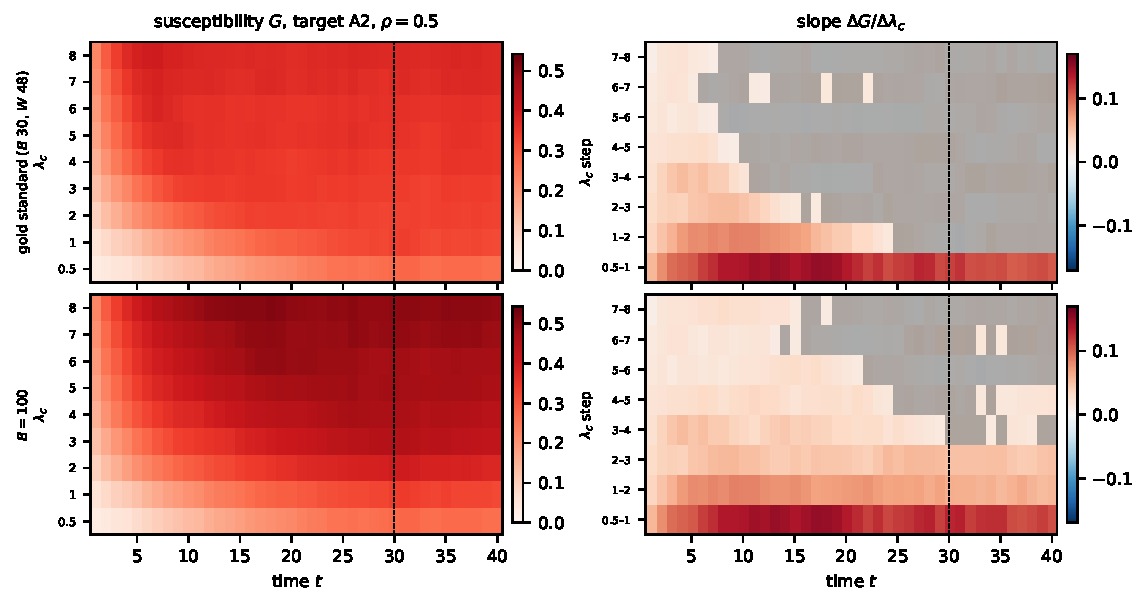
\includegraphics[width=0.9\linewidth]{figures/fig_strength_time_budget.pdf}
\caption{$G$, target A2 (left), and its slope between neighbouring rates (right) over time and rate, $\rho = 0.5$.
Faded cells: the paired 95\% interval of the slope includes 0.}
\label{fig:strengthtimeB}
\end{figure}

\begin{itemize}\itemsep1pt
\item \textbf{With $B = 100$ more rate keeps paying on $t = 30$} (Figure~\ref{fig:strengthB}): at $\rho = 0.5$ the steps
  up to $\lambda_c = 3$ are significant ($+0.13$, $+0.06$, $+0.05$ per unit of rate); in the gold standard only the
  first ($+0.12$).
\item \textbf{The budget moves the controller along one curve} (Figure~\ref{fig:messagesB}): with 30 messages the gold
  standard's points pile up at the budget; with 100 they continue the same rising curve, from 0.33 (24 messages) to
  0.50 (78 messages) at $\rho = 0.5$.
\item \textbf{Over time} (Figure~\ref{fig:strengthtimeB}): in the gold standard the steps above $\lambda_c = 1$ fade
  between $t \approx 5$ and 25; with $B = 100$ those up to $\lambda_c = 3$ stay positive to $t = 30$.
\item Gate off minus on: $-0.01$ to $+0.04$, as in the gold standard.
\end{itemize}

\subsection{Who holds the proof}

\begin{figure}[H]
\centering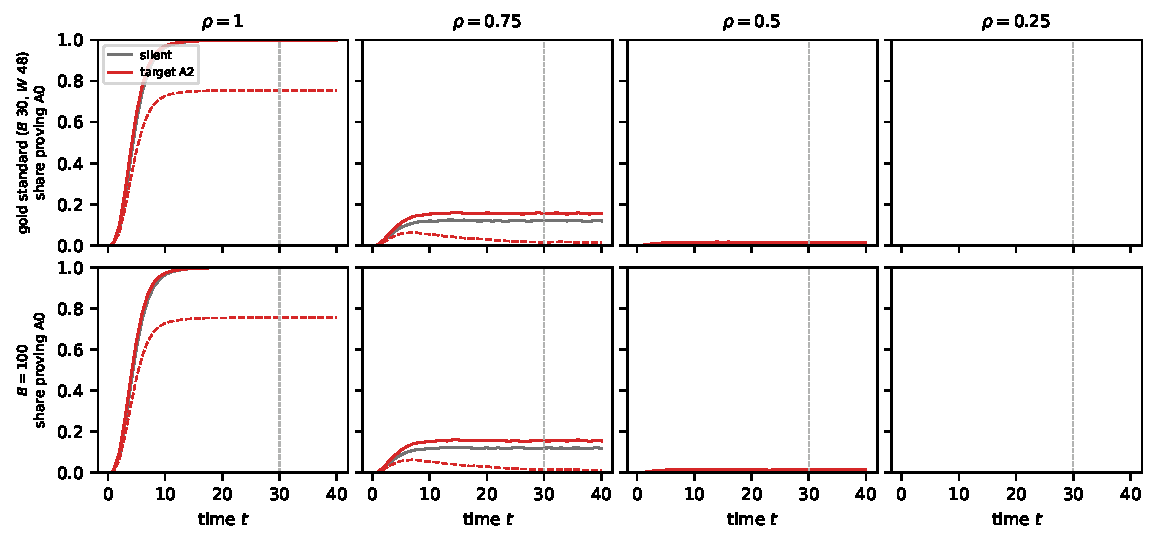
\includegraphics[width=0.98\linewidth]{figures/fig_proofs_budget.pdf}
\caption{Share of agents whose remembered facts prove A0 (solid) and who prove it from their original facts only
(dashed), without a controller (grey) and with the false controller at $\lambda_c = 1$ (red); columns $\rho$.}
\label{fig:proofsB}
\end{figure}

At $\lambda_c = 1$ the budget does not change who holds the proof: at $\rho = 1$ all agents prove A0, 76\% from their
own facts (100\% without a controller); at $\rho \le 0.5$ at most 2\%.

\paragraph{What the budget changes.} A larger budget raises the false controller's end point by up to 0.13
($\rho \le 0.5$), up to 0.06 at $\rho = 0.75$ and nothing at $\rho = 1$, with each extra message worth about half as
much. The gold standard's ``the budget sets the end point and the rate sets the speed'' becomes: \emph{faster rates
and larger budgets both raise the end point, with diminishing returns per message; the 30-message cap is what made
the rate look irrelevant}.

%=====================================================================================================================
\section{Part B: a board that forgets faster or slower ($W = 24$, $W = 240$)}\label{sec:window}

$W = 24$ (posts readable for about 1 time unit), the gold standard ($W = 48$, about 2) and $W = 240$ (about 10);
the budget is $B = 30$ in all three.

\subsection{Votes over time}

\begin{figure}[H]
\centering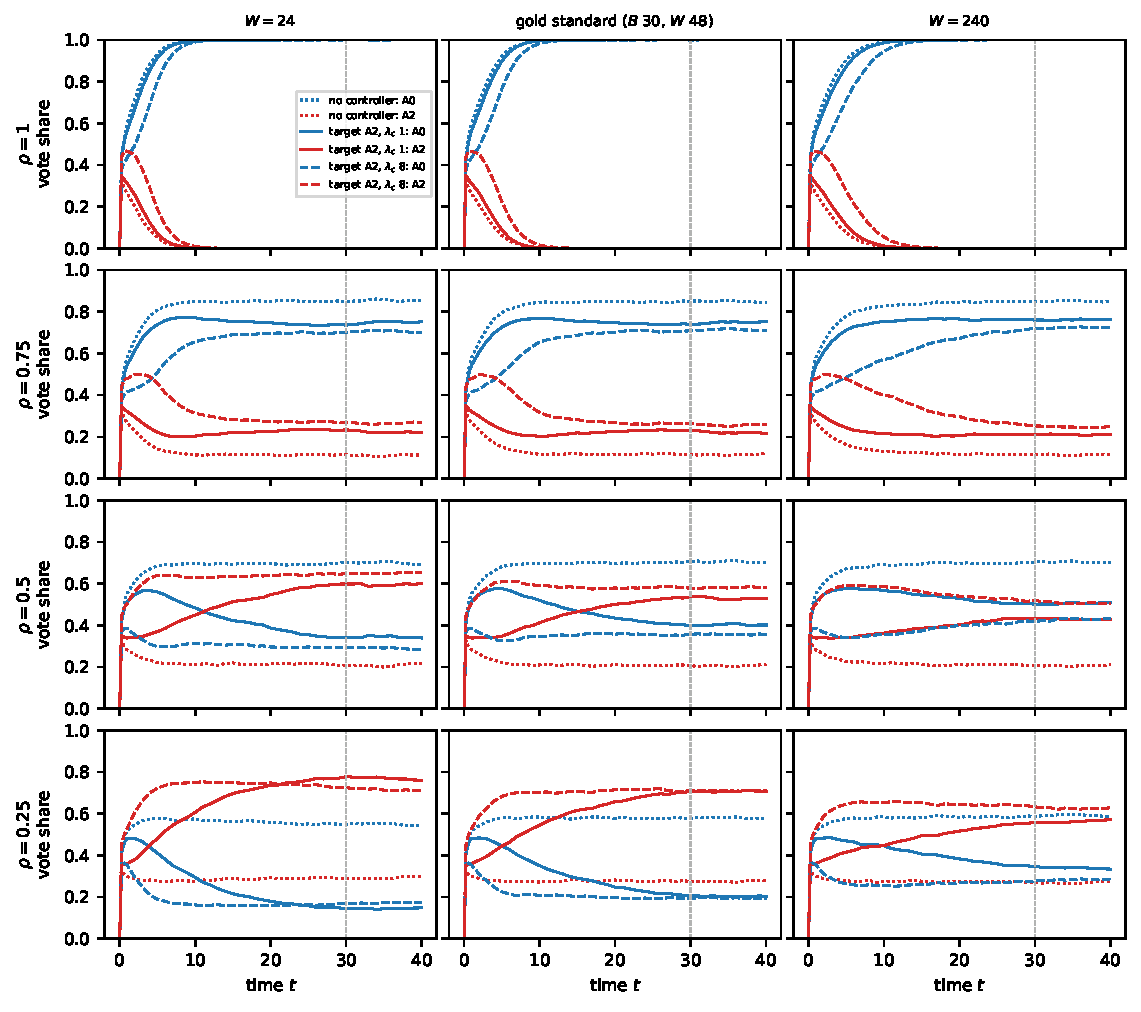
\includegraphics[width=0.78\linewidth]{figures/fig_votes_window.pdf}
\caption{As Figure~\ref{fig:votesB}, for the three windows.}
\label{fig:votesW}
\end{figure}

\begin{itemize}\itemsep1pt
\item \textbf{Without a controller the window hardly matters}: the shares on $t = 30$ differ by at most 0.03.
\item \textbf{With full memory every window is immune}: A2 is back to 0 by $t = 30$.
\item \textbf{A longer window protects}: A2 on $t = 30$ at $\lambda_c = 1$ is 0.60, 0.54 and 0.43 for $W = 24$, 48, 240
  at $\rho = 0.5$, and 0.78, 0.71, 0.56 at $\rho = 0.25$; at $\lambda_c = 8$, 0.65, 0.58, 0.52 and 0.73, 0.71, 0.63.
\end{itemize}

\subsection{Susceptibility over time, and per message}

\begin{figure}[H]
\centering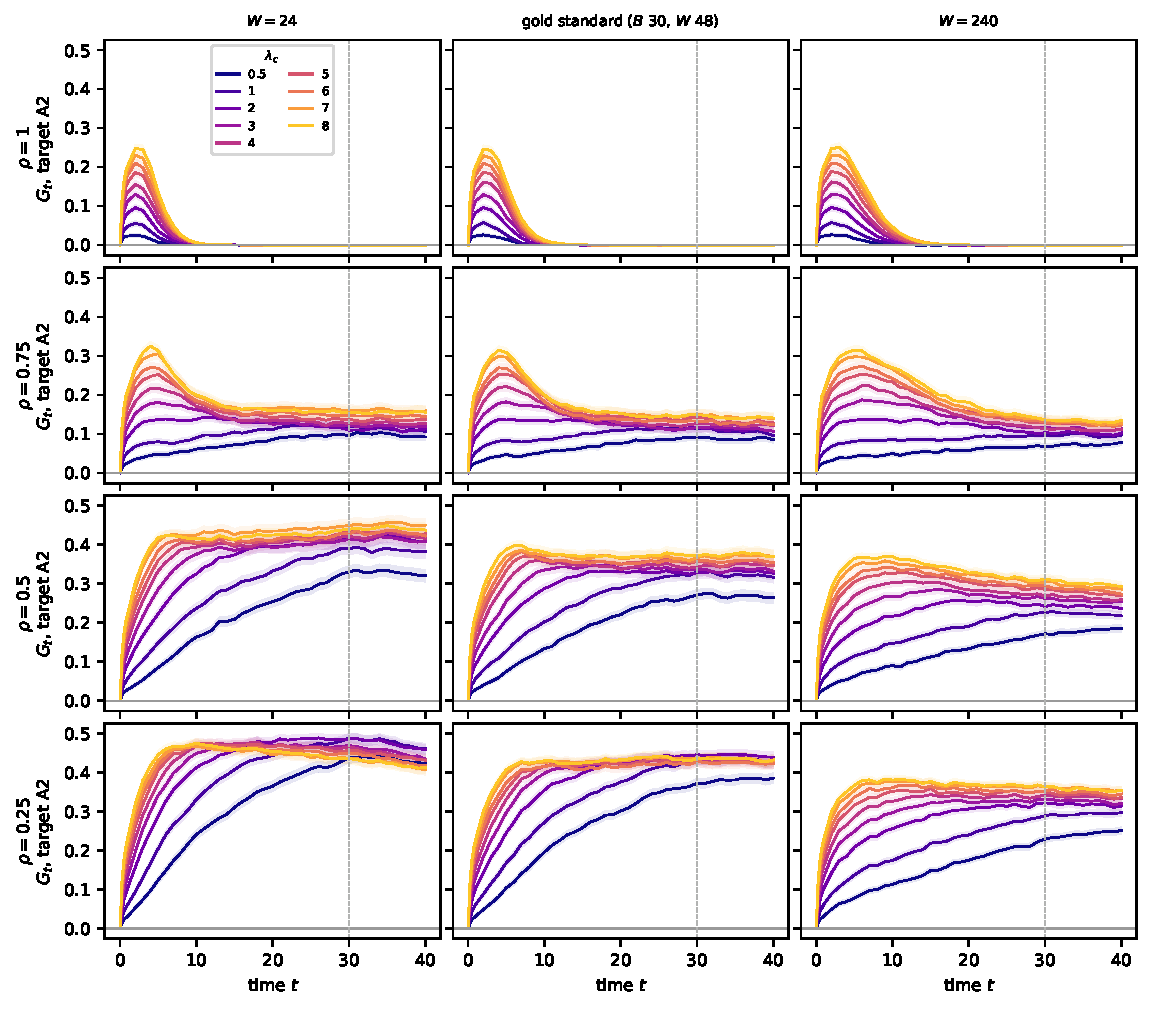
\includegraphics[width=0.78\linewidth]{figures/fig_gain_time_window.pdf}
\caption{Paired susceptibility $G_t$, target A2, one curve per rate (bands: 95\% intervals).}
\label{fig:gainW}
\end{figure}

\begin{figure}[H]
\centering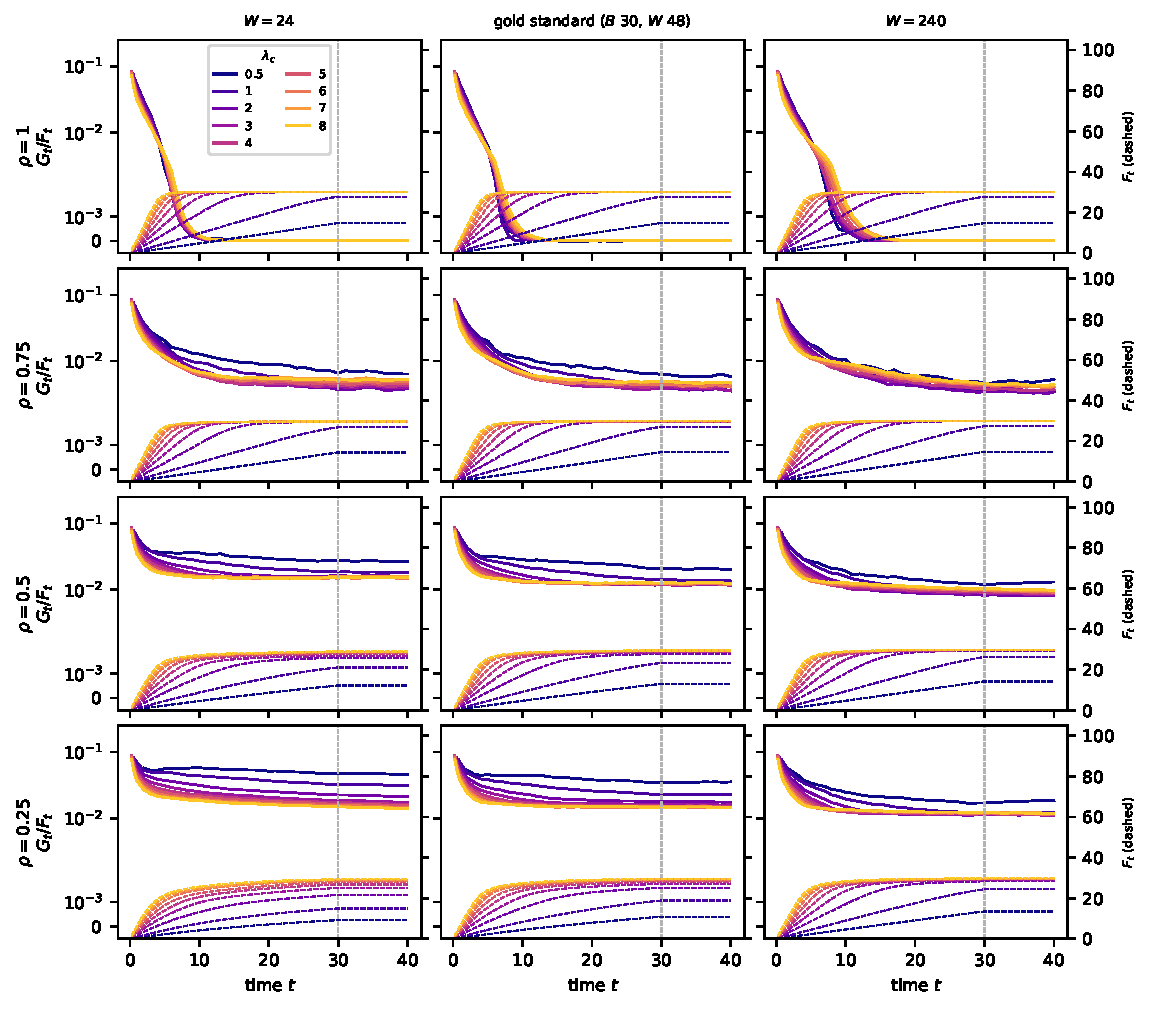
\includegraphics[width=0.78\linewidth]{figures/fig_per_fact_window.pdf}
\caption{Gain per message $G_t/F_t$ (solid) and messages posted $F_t$ (dashed), target A2, one colour per rate.}
\label{fig:perfactW}
\end{figure}

\begin{itemize}\itemsep1pt
\item \textbf{$W = 24$ raises $G$, $W = 240$ lowers it, at every rate} (Figure~\ref{fig:gainW}): on $t = 30$, $\rho = 0.5$:
  0.33--0.45, 0.27--0.37, 0.17--0.31 for $W = 24$, 48, 240; $\rho = 0.25$: 0.44--0.49, 0.37--0.45, 0.23--0.36. Rate by
  rate, $W = 240$ lowers $G$ by 0.06--0.14 at $\rho \le 0.5$ and $W = 24$ raises it by up to 0.09; at $\rho = 0.75$ both
  change it by at most 0.03. With $W = 240$ fast controllers peak early and fade ($\rho = 0.5$, $\lambda_c = 8$: 0.37
  at $t = 5$, 0.31 at $t = 30$).
\item \textbf{Readability follows} (Figure~\ref{fig:phaserxW}, middle): on $t = 30$, $\rho = 0.5$, $I = 0.20$--$0.34$,
  0.15--0.27, 0.09--0.21 bits. \textbf{The efficiency does not move} (right): $\eta = 0.78$--$0.93$ at $\rho < 1$ for
  every window.
\item \textbf{Each message is worth more when the board forgets fast} (Figure~\ref{fig:perfactW}): at $\lambda_c = 1$,
  $\rho = 0.25$: 0.033, 0.023 and 0.012 per message.
\end{itemize}

\subsection{Phase diagrams}

\begin{figure}[H]
\centering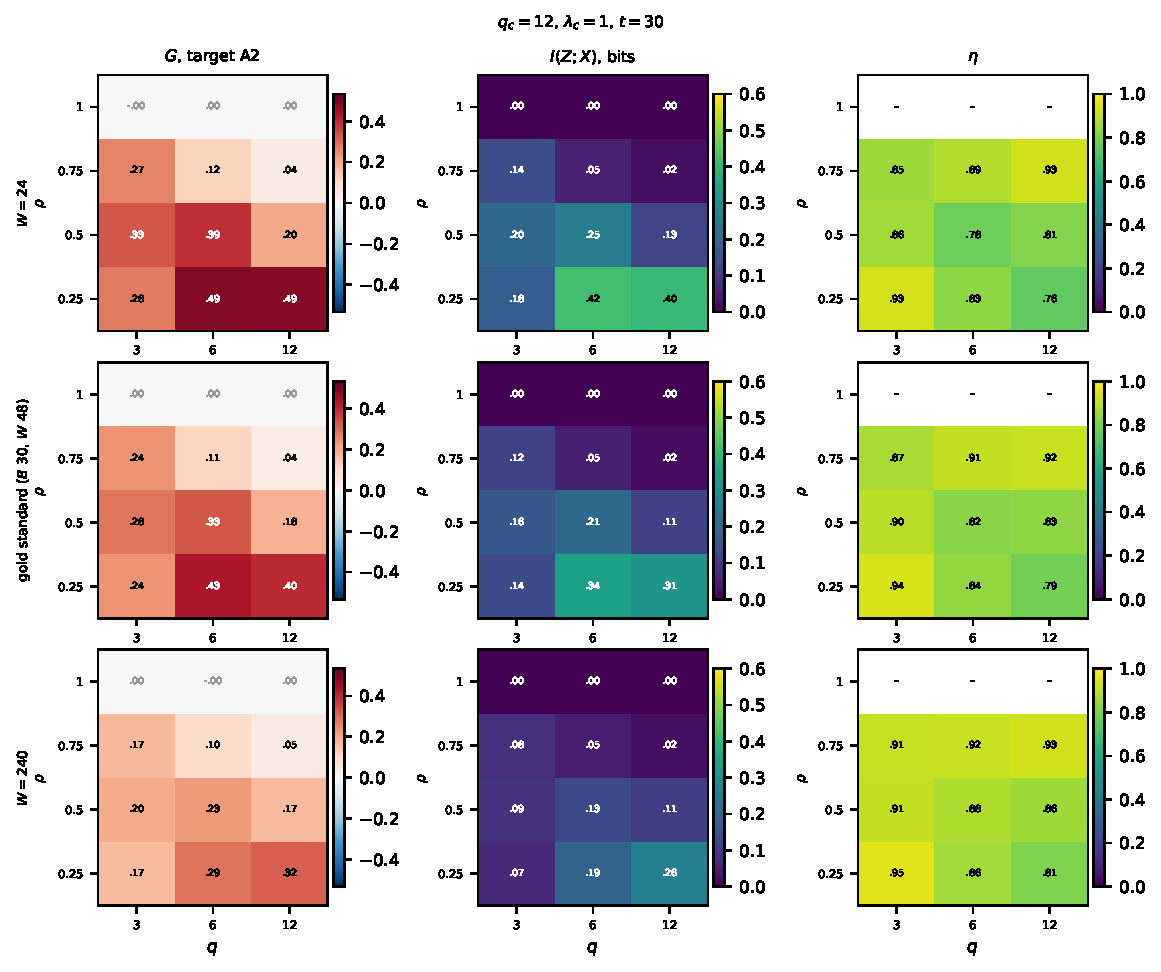
\includegraphics[width=0.9\linewidth]{figures/fig_phase_rho_q_window.pdf}
\caption{As Figure~\ref{fig:phaserqB}, for the three windows.}
\label{fig:phaserqW}
\end{figure}

\begin{figure}[H]
\centering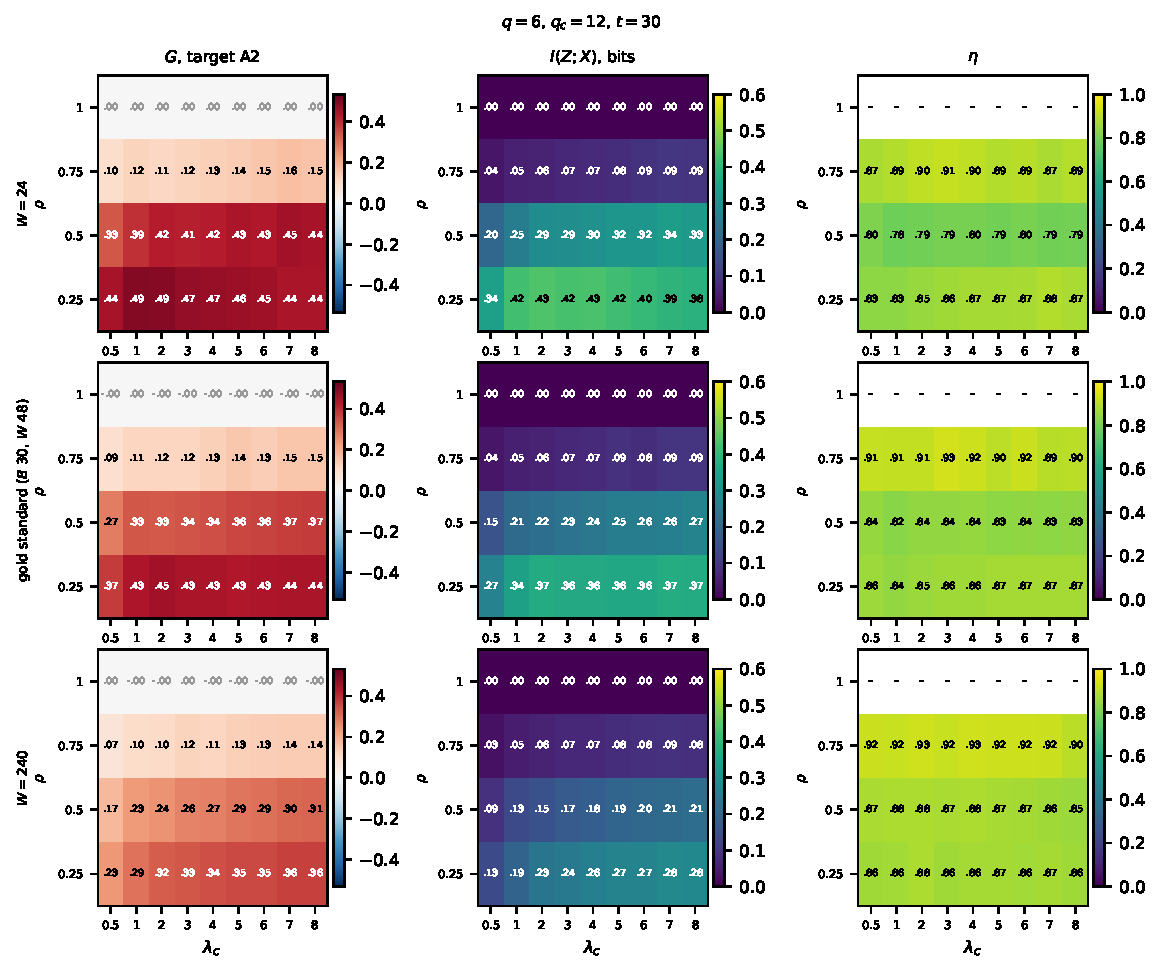
\includegraphics[width=0.9\linewidth]{figures/fig_phase_rho_x_window.pdf}
\caption{As Figure~\ref{fig:phaserxB}, for the three windows.}
\label{fig:phaserxW}
\end{figure}

\begin{itemize}\itemsep1pt
\item \textbf{The reading reversal survives every window} (Figure~\ref{fig:phaserqW}), smaller with $W = 240$: from
  $q = 3$ to 12, $G$ falls at $\rho = 0.75$ (0.27 $\to$ 0.04, 0.24 $\to$ 0.04, 0.17 $\to$ 0.05 for $W = 24$, 48, 240) and
  rises at $\rho = 0.25$ (0.28 $\to$ 0.49, 0.24 $\to$ 0.40, 0.17 $\to$ 0.32).
\item \textbf{Memory stays the main axis} (Figure~\ref{fig:phaserxW}). $W = 240$ adds a weak rate gradient (from
  $\lambda_c = 1$ to 8: $+0.09$ at $\rho = 0.5$, $+0.07$ at $\rho = 0.25$); $W = 24$ none ($+0.05$, $-0.05$).
\end{itemize}

\subsection{Susceptibility against the rate, against messages, and its slope}

\begin{figure}[H]
\centering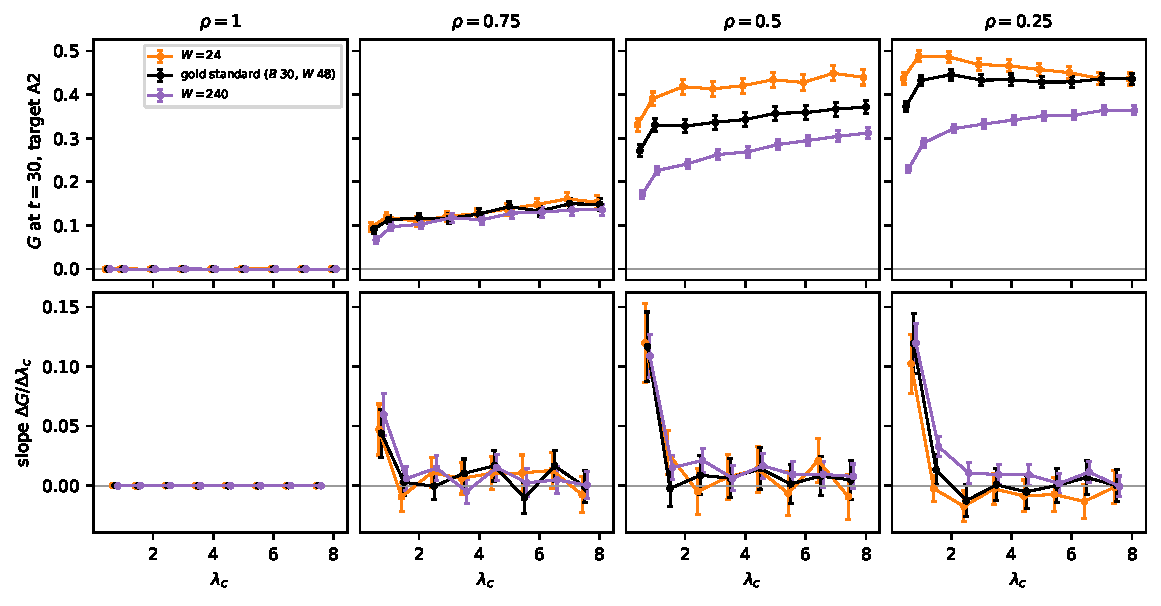
\includegraphics[width=0.98\linewidth]{figures/fig_gain_rate_window.pdf}
\caption{As Figure~\ref{fig:strengthB}, for the three windows.}
\label{fig:strengthW}
\end{figure}

\begin{figure}[H]
\centering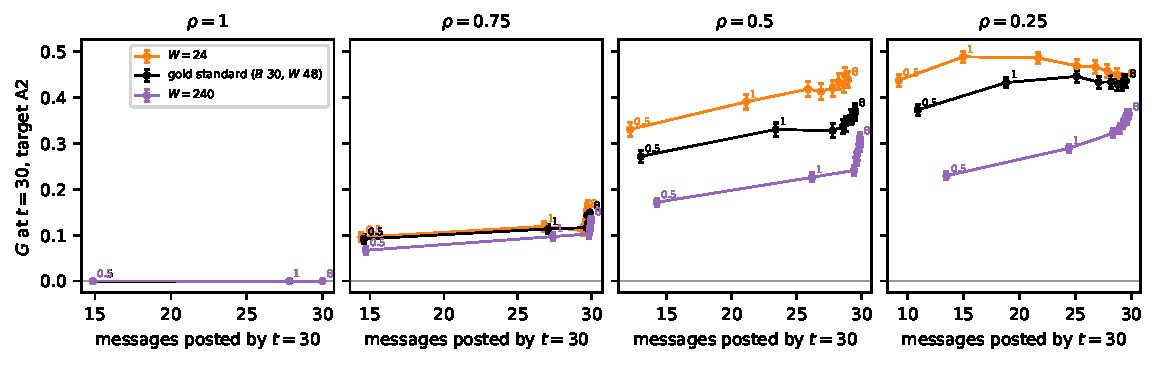
\includegraphics[width=0.98\linewidth]{figures/fig_gain_messages_window.pdf}
\caption{As Figure~\ref{fig:messagesB}, for the three windows.}
\label{fig:messagesW}
\end{figure}

\begin{figure}[H]
\centering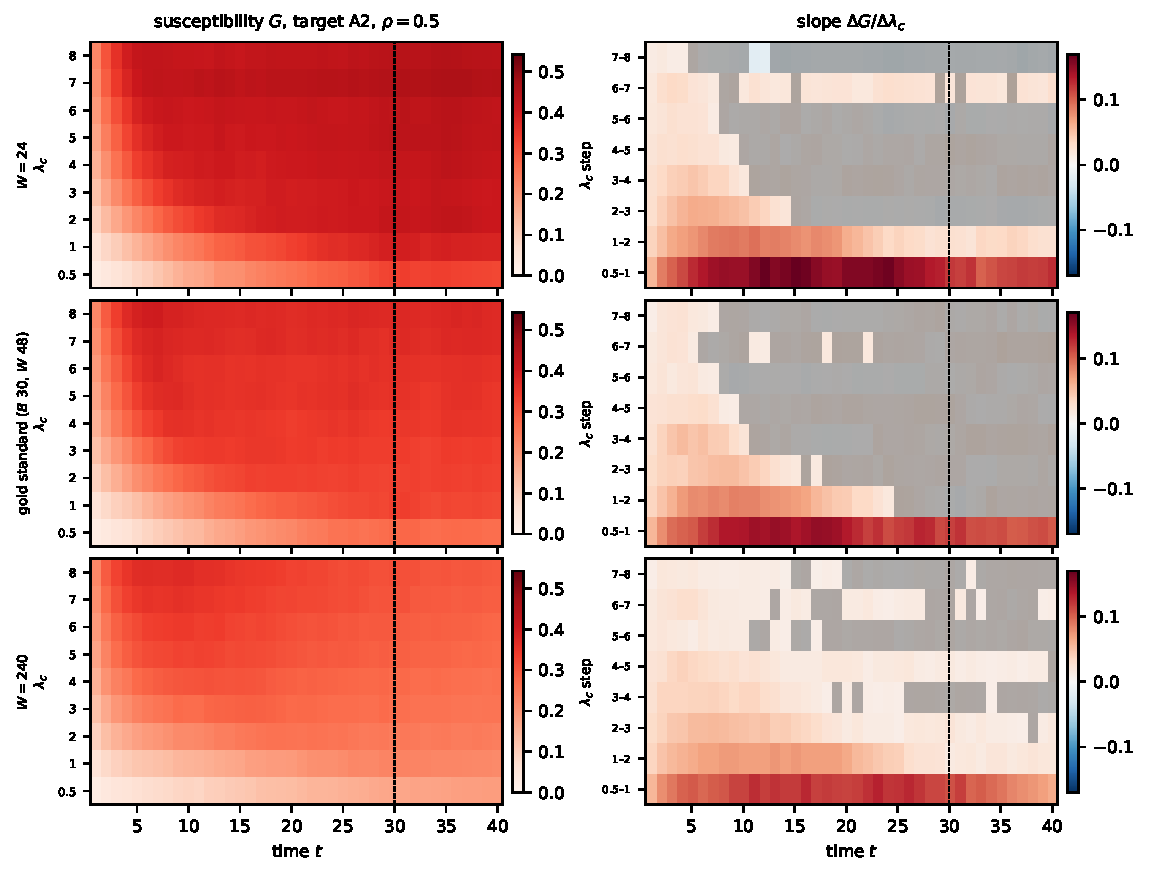
\includegraphics[width=0.9\linewidth]{figures/fig_strength_time_window.pdf}
\caption{As Figure~\ref{fig:strengthtimeB}, for the three windows.}
\label{fig:strengthtimeW}
\end{figure}

\begin{itemize}\itemsep1pt
\item \textbf{The window moves the whole curve} (Figure~\ref{fig:messagesW}): every window posts about the same
  messages, but at the same 28--30 messages $G$ is 0.45 ($W = 24$), 0.37 ($W = 48$) and 0.31 ($W = 240$) at
  $\rho = 0.5$.
\item \textbf{The slopes look like the gold standard's} (Figures~\ref{fig:strengthW}, \ref{fig:strengthtimeW}): the first
  step dominates ($+0.10$ to $+0.12$ at $\rho \le 0.5$); with $W = 240$ a few later steps are also slightly positive
  (up to $+0.03$).
\item Gate off minus on: $-0.03$ to $+0.03$ for every window.
\end{itemize}

\subsection{Who holds the proof}

\begin{figure}[H]
\centering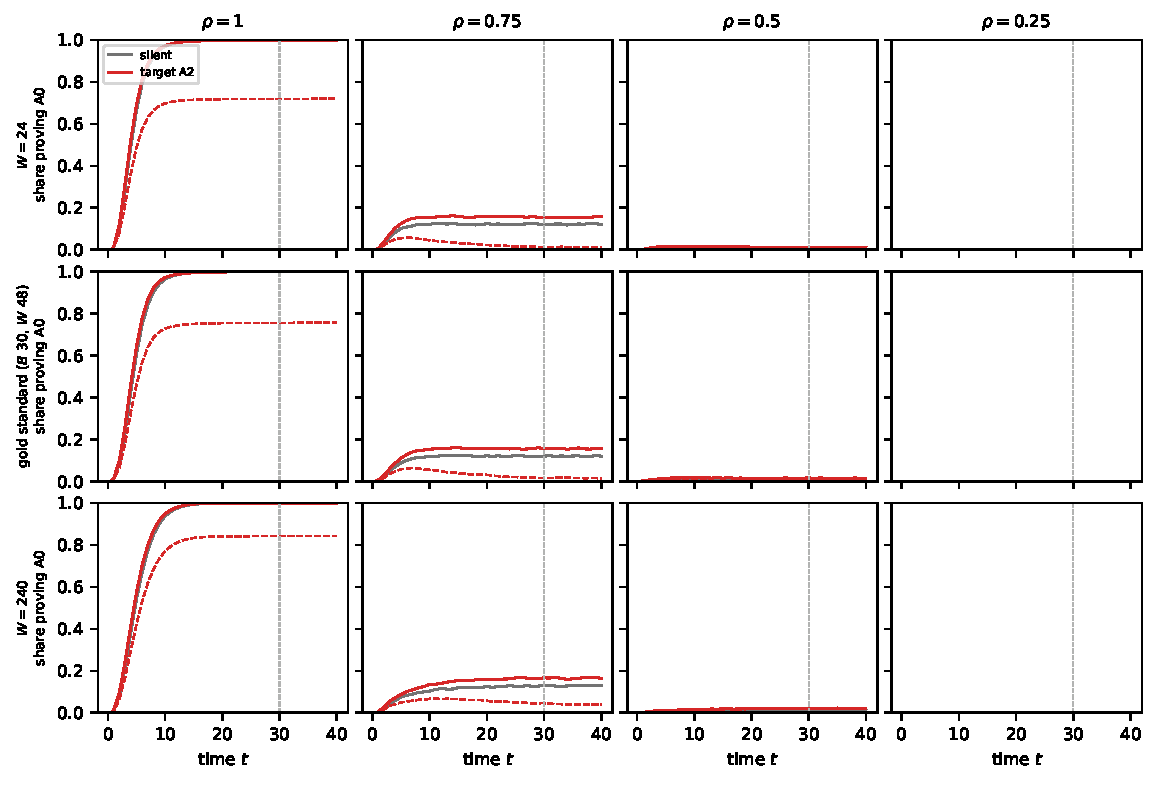
\includegraphics[width=0.98\linewidth]{figures/fig_proofs_window.pdf}
\caption{As Figure~\ref{fig:proofsB}, for the three windows.}
\label{fig:proofsW}
\end{figure}

Only full memory keeps the proof, for every window. At $\rho = 1$ the window changes how many proofs stay the agents'
own under the false controller: 72\% ($W = 24$), 76\% ($W = 48$), 84\% ($W = 240$).

\paragraph{What the window changes.} The board's memory protects like the agents' memory, but less: keeping posts
readable for 10 time units instead of 2 lowers the false controller's gain by 0.06--0.14 at $\rho \le 0.5$, keeping
them 1 time unit raises it by up to 0.09, while the agents' memory $\rho$ moves it by up to 0.43. A likely reason,
not tested: a long window keeps the agents' older posts, which carry the facts of the proof, readable for longer.

%=====================================================================================================================
\section{Conclusions}

\begin{enumerate}\itemsep2pt
\item \textbf{The main results of the gold standard hold in all three variants}: full memory makes the swarm immune;
  forgetting makes it steerable; reading more protects when agents remember and helps the controller when they
  forget; the gate matters little.
\item \textbf{The budget}: more messages raise the end point with diminishing returns, only where the swarm is
  already steerable (Part~A).
\item \textbf{The board's memory}: a longer window protects the swarm, a shorter one exposes it; smaller effects than
  the agents' memory (Part~B).
\item \textbf{The controller targeting A0} is left out of this report: in every variant its gain on $t = 30$ stays
  within 0.03 of the gold standard's, because the vote gate keeps it mostly silent (1--29 messages by $t = 30$).
\end{enumerate}

\paragraph{Caveats.} The window changes what the controller reads too: with $W = 240$ its vote gate sees votes up to
10 time units old, and at $\lambda_c = 1$ it posts 24--28 messages instead of 19--28. The variants were run at
$q_c = 12$ and four memory values only, so the gold standard's $q_c \times \lambda_c$ diagram has no counterpart. One
world, 24 exact-Bayesian agents, one controller policy; 1{,}000 episodes per setting (95\% intervals on $G$ about
$\pm 0.02$). Data: \texttt{results/simulation\_2/2026-10-18\_sim2\_symmetric\_*}; tables:
\texttt{results/gold\_standard/2026-10-18/} (variants) and \texttt{2026-10-16/} (gold standard); code:
\texttt{shared\_analysis/gold\_standard/make\_report\_figures\_2026-10-19.py}.

\end{document}
